\chapter{\textbf{Conclusions and Future Work}}
This work described the development of a deeply-integrated flight vehicle dynamic model within a GPS L1 C/A vector tracking software defined receiver. A performance analysis of the proposed navigation filter in GPS-challenged environments compared to the standard VDFLL was presented. The work presented in this thesis extends the state of the art by modeling a flight vehicle dynamic model deeply-coupled with GPS correlator measurements. The fidelity of the model stems from multiple flight mechanic modules presented in Chapter 2. The aerodynamic module models aerodynamic forces and moments on the basis of strip theory, using pre-processed CFD tables to propagate the aerodynamic coefficients based on the current flight condition of the aircraft. The engine and propeller module comprise of pre-processed numerical tables based on historical engine and propeller data sheets and performance charts. The FVDM improves the extended Kalman filter time update by fully acknowledging the behavior of the presented flight vehicle {--} this can be cumbersome with hardware sensors such as an IMU or barometer. The presented FVDM can be run at any update frequency, typically a limiting factor for hardware sensors. An increased update frequency for any vehicle dynamic model increases the likelihood that changes in the states are linear between time steps, this is especially important for high-dynamic systems such as hyper-velocity vehicles. Unlike hardware sensors, the FVDM is not subject to vibration, which is a common amongst rotor craft and fixed-wing flight vehicles. The downside to the FVDM is the requirement to have extensive knowledge of the flight vehicle in order to model it with high fidelity. This can be difficult if modeling government or proprietary vehicles.

For the straight, constant altitude trajectory, the proposed navigation filter was shown to have comparable results to that of the standard constant-velocity VDFLL implementation. However, when given a more dynamic trajectory, the deeply-integrated FVDM shows improvement by at least double in all scenarios of signal degradation. This is partly due to the FVDM being able to estimate the angular rate and Euler attitude of aircraft, where as the standard VDFLL implementation does not have this capability.

% \section{\textbf{Concerns of Observability}}

% From the presented navigation filter, measurements of position and velocity appear in the form of pseudorange and pseudorange-rates. These measurements are created based on DLL and FLL discriminator outputs that are converted to meters and meters per second, respectively. When a measurement update occurs within the EKF, these measurements indirectly correct the current state estimate through a the observation matrix, \(\mathbf{H}\) (Equation~\ref{eq:H}). As stated previously, one reason for faulty estimates of the aircraft in GPS-denied environments is the lack of observability in the angular states. Once the estimated angular rates of the aircraft drift, and through integration, their respective Euler angles, the FVDM will continue to propagate the aircraft with these drifting estimates. For example, if the pitch angle estimate of the FVDM starts to drift from 10 degrees to 20 degrees to 30 degrees, the aircraft will naturally begin to pitch up and gain altitude. If the VT algorithm loses lock with signal channels, or the channel measurements are poor, there is no other measurements to correct the FVDM and it will continue to propagate worse estimates of the state. This can be further examined by exploring the observability matrix, \(\mathbf{O}\) through time.

% \begin{equation}\label{eq:O}
%     \mathbf{O} = \begin{bmatrix}
%         \mathbf{H}_k                    \\
%         \mathbf{H}_k\mathbf{\Phi}_k       \\
%         \mathbf{H}_k\mathbf{\Phi}_k^2     \\
%         \mathbf{H}_k\mathbf{\Phi}_k^3     \\
%         \vdots                        \\
%         \mathbf{H}_k\mathbf{\Phi}_k^{n-1} \\
%     \end{bmatrix}
% \end{equation}

% A system is fully-observable if the all of the states of the system can be known by the outputs of the systems, that is, if the rank of Equation~\ref{eq:O} is equal to the number of states in \(\mathbf{X}\) (Equation~\ref{eq:stateVector}), then the observability matrix is full rank and the system is fully-observable. A quick calculation of \(\mathbf{O}\) shows that the deeply-coupled FVDM is not fully-observable. 


\section{\textbf{Future Work}}
For future work, the author recommends several items, both relating to the proposed navigation filter and to components of the FVDM presented in this work. With the complexity of the model, a common question is asked: \textit{What level of fidelity is needed to acquire accurate estimates?} To answer this question, a new architecture of the FVDM is theorized (Figure~\ref{fig:futurework}), with its benefits listed herein. 
\begin{figure}[!ht]
    \centering
    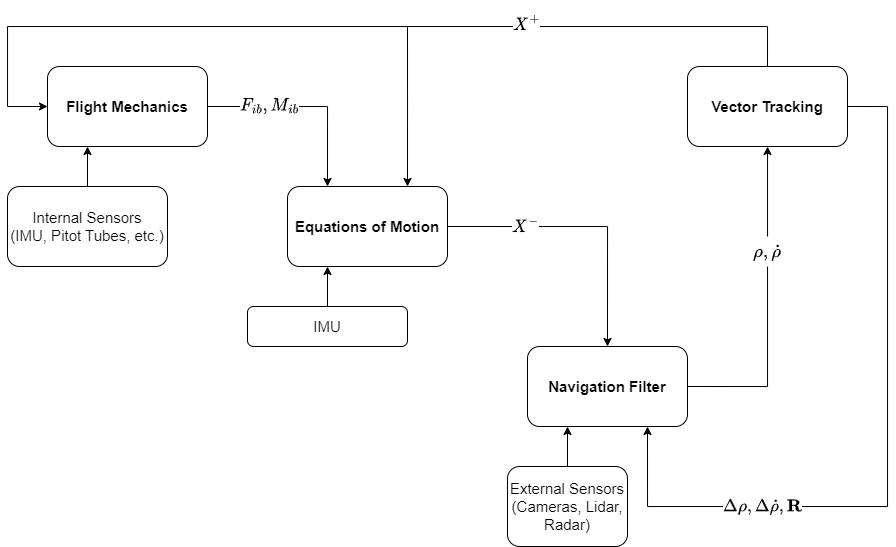
\includegraphics[width=\linewidth]{Figures/futurework.drawio.png}
    \caption{Cascaded architecture for an improved FVDM coupling.}\label{fig:futurework}
\end{figure}
One of the downsides to the presented FVDM is the extremely catered modeling of one aircraft, the Diamond DA-40. The cascaded architecture would improve this such that aerodynamic coefficients are estimated inside of the flight mechanics module instead of being compiled beforehand using a CFD program. This would make the FVDM more generalizable, theoretically allowing it to be applicable to any aircraft, barring any configuration differences. The second improvement would be the fusion of other available sensors with the FVDM\@. For the presented work, it was assumed that the sensor suite became faulty or the size of the flight vehicle limited the capacity in which it could carry sensors. In reality, the form factor of modern low-cost sensors allow them to fit within the casing of a smart phone, and as such, should be fused with the FVDM for better estimates of forces and moments acting onto the airframe. Typically, low-cost sensors are unable to update at high frequencies, discouraging their use onto high-dynamic systems. However, the FVDM is able to run at higher frequencies, so a fusion between the FVDM and low-cost sensors is intriguing and possible with the cascaded architecture. If fusing multiple sensors with the FVDM using the cascaded architecture, it would be possible to measure the effectiveness of each sensor. Through decades of prior research, multi-sensor fusion algorithms have shown to provide robust pose estimates of the collection platform for a variety of dynamics and signal interference. The cascaded architecture proposed in this section would allow further fusion of sensors not typically used in navigation algorithms (i.e.\ pitot tubes, engine temperature sensor) via the modeling equations from the FVDM\@.



